% !TeX root = ../main.tex

\subsection{Chromatin Coarse-Graining, chromatin as a polymeric fluid}

The Young's modulus ($E$) of a chain is the extent to which a solid material (or a polymeric fluid, in this case) can be deformed
As Robert Hook noticed, the following is valid 
\begin{equation}
    \sigma = E \frac{\Delta l}{l}
\end{equation}
Where $l$ represents the length of the chain and $\Delta l$ the deformation $\sigma$
\cite{grosbergGiantMoleculesHere2011}

The entanglement length ($N_e$) corresponds to the Young's modulus that is experimentally found in the plateau region where a force starts to produce irreversible deformations in a chain.

% #TODO put a reference image if you want


It is also defined as the "the average number of monomer units along the chain between two nearest effective cross-links."
and is related to the ability of chains to form knots between each other
\cite{grosbergGiantMoleculesHere2011}
.

%#TODO add subchapter rosettes


\subsubsection{Persistence length of a polymer chain}
%#TODO add subchapter persistence length

The persistence length (\textit{PL}) of a polymer represents the degree of bendability of the chain. During this project, the persistence length is shown in equation \ref{eq: persistence length}.


\begin{equation}
    PL = lk_{CG} / b_{CG} / 2
\end{equation}

With the idea of following a "journey" on the polymer chain, the average angle that you obtain at a contour length $s$ is as in equation \ref{eq: contour length mean angle}. In general, the lower is the contour length analyzed with respect to the persistance length, the higher is the probability of having a low degree angle ($\cos{\theta} \sim 1$). On the contrary, by analyzing larger lengths, it is possible to obtain a wider range of angles.
The concept of persistance length is used in the polymer model to compute the angle bending potentials, which is calculated as in equation \ref{eq: angle bending potential}.


\begin{equation} \label{eq: contour length mean angle}
    \langle \cos{\theta(s)}\rangle = \exp{\left(-\frac{s}{l}\right)}
\end{equation}

\begin{figure}[H] 
    \centering 
    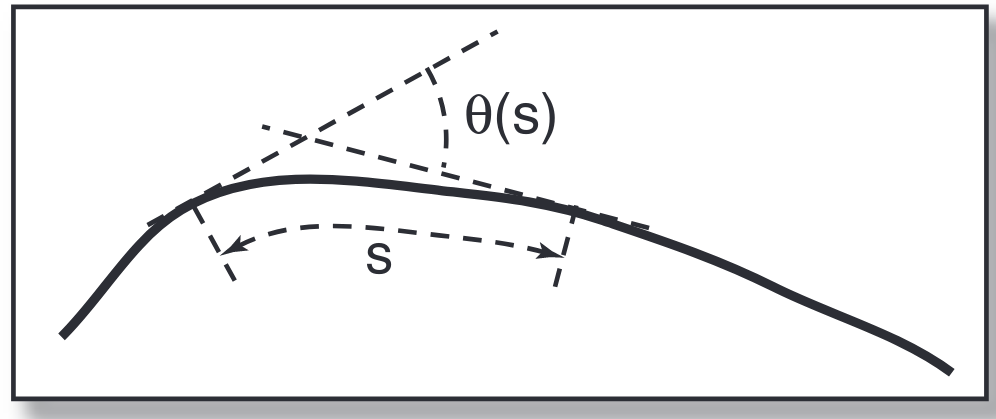
\includegraphics[width=75mm]{persistance_length.png} 
    \caption{Image taken from Grosberg \textit{et al.} 2011\cite{grosbergGiantMoleculesHere2011}. Angle formed between the extremes of a contour length.} 
    \label{examplelabel} 
\end{figure}

%#TODO about the reason of coarse graining with such a low resolution
%#TODO fine scale e coarse grained model, explain reasons
